%----------------------------------------------------------------------------------------
%	PACKAGES AND OTHER DOCUMENT CONFIGURATIONS
%----------------------------------------------------------------------------------------

\documentclass{article}

\input{structure.tex} % Include the file specifying the document structure and custom commands

\usepackage{hyperref}

\usepackage[T1, T2A]{fontenc} % Output font encoding for international characters

\usepackage{siunitx}

\usepackage{xcolor} % to color the conversation to look better

\usepackage{amsmath}


\title{High Precision Bandgap Reference Voltage}

\author{Aleksandar Vuković}

% \author[2,3]{Second Author}
% \author[2]{Third Author}
% \affil[1]{First Department, First University, First Country}
% \affil[2]{Institute Name, Second Country}
% \affil[3]{Third Department, Third Affiliation, Third Country}

\date{}

\begin{document}

\maketitle

\begin{abstract}
    Includes specifications for the block. Different topologies for Bandgap and Opeational Transconductace Amplifier. 

    \textbf{Keywords:} high precision, trimming, Kuijk, Brokaw, Tsividis, bandgap, voltage reference, OTA
\end{abstract}

\section{Topoplogy classification}

There are three basic types of Bandgap Voltage References based on % \parencite{krolak2022}: 

\begin{itemize}
    \item Kuijk Bandgap
    \item Brokaw Bandgap
    \item Tsividis Bandgap
\end{itemize}

\subsection{Kuijk Bandgap} % Mathematical Behaviour :/

\begin{figure}[ht!]
	\centering
	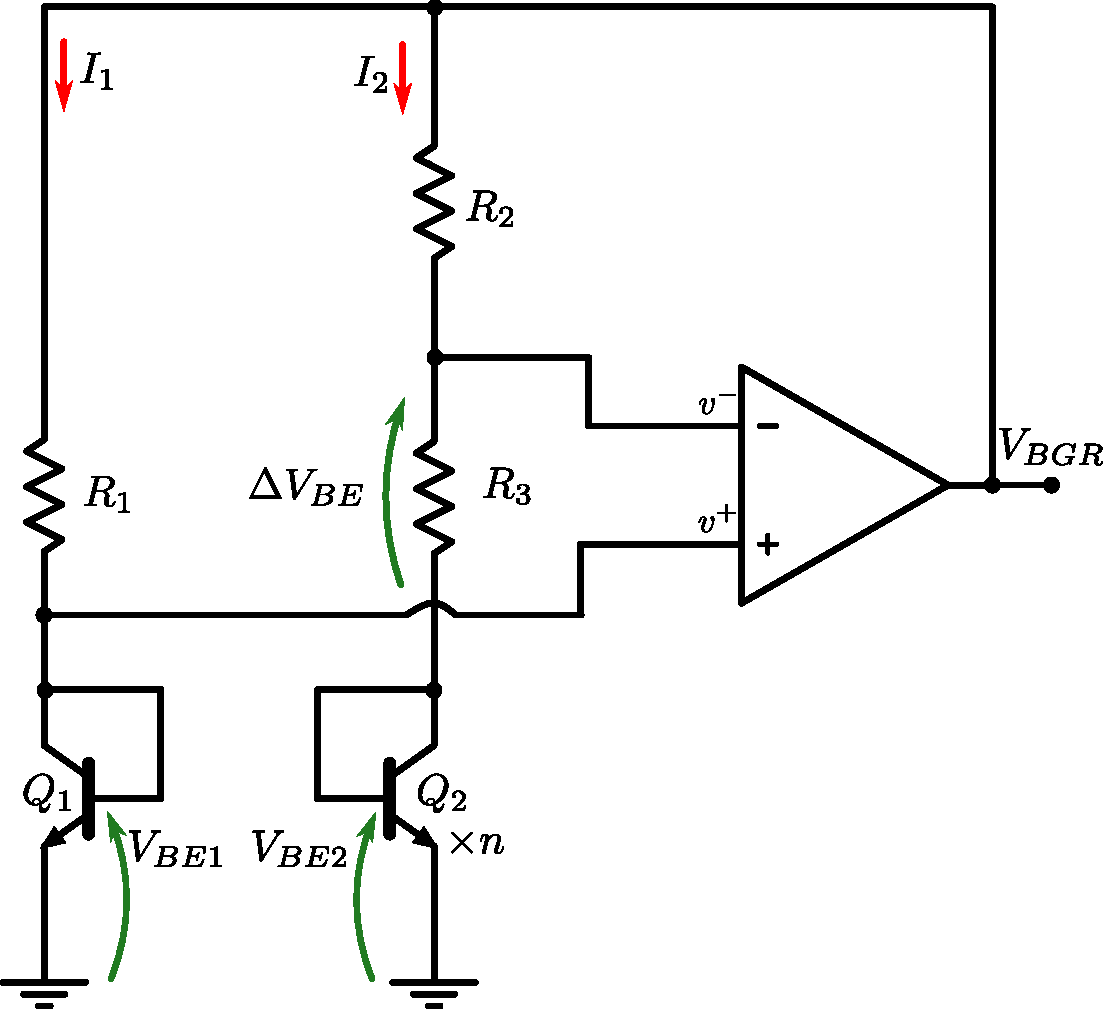
\includegraphics[width=0.55\linewidth]{Figures/BGRV-Kuijk.pdf}
	\caption{Kuijk Bandgap Reference Voltage}
	\label{fig:kuijk} % !?
\end{figure}

This design is based on Kuijk paper from 1972.

\begin{equation}\label{eq:id1}
    I_{C1} = I_{s1} (e^{V_{BE1}/V_T}-1) \, ; \, V_{BE1} = V_T ln(\frac{I_{C1}}{I_s})
\end{equation}

\begin{equation}\label{eq:id2}
    I_{C2} = I_{s2} (e^{V_{BE2}/V_T}-1)
\end{equation}

Because of scaling $A_E$

\begin{equation}
    I_{s2} = n \, I_{s1}
\end{equation}

Saturation current is defined as:

\begin{equation}
    I_{sn} = q n_i^2 A_E \dfrac{D_{n,B}}{N_B w'_B}
\end{equation}

Divide current equations \ref{eq:id1} and \ref{eq:id2}:

\begin{equation}
    n \dfrac{I_{D1}}{I_{D2}} = e^{(V_{BE1} - V_{BE2})/V_T}
\end{equation}

\begin{equation}
    V_{BE2} - V_{BE1} = \dfrac{kT}{q} ln (\dfrac{n I_{D1}}{I_{D2}})
\end{equation}

This difference is applied on resistor $R_3$.

\begin{equation}
    \dfrac{\Delta V_{BE}}{R_3} = \dfrac{V_{BGR} - V_{BE1}}{R_2} = \frac{1}{R_3}\dfrac{kT}{q} ln (\dfrac{n I_{D1}}{I_{D2}})
\end{equation}

\begin{equation}
    V_{BGR} = V_{BE1} + \Delta V_{BE} \dfrac{R_2}{R_3}
\end{equation}

If we approximate that $I_{D1} \approx I_{D2}$ :

\begin{equation}
    V_{BGR} = V_{BE1} +  \dfrac{kT}{q} ln (n) \dfrac{R_2}{R_3}
\end{equation}

Mathematical equation for $I_{C1}$.

% \subsubsection*{Equality of $I_{c1}$ and $I_{c2}$ }
\begin{equation}
    V_{BGR} - V_{BE1} = R_1 I_{C1}
\end{equation}

\subsection{Brokaw bandgap reference}

\begin{figure}[ht!]
	\centering
	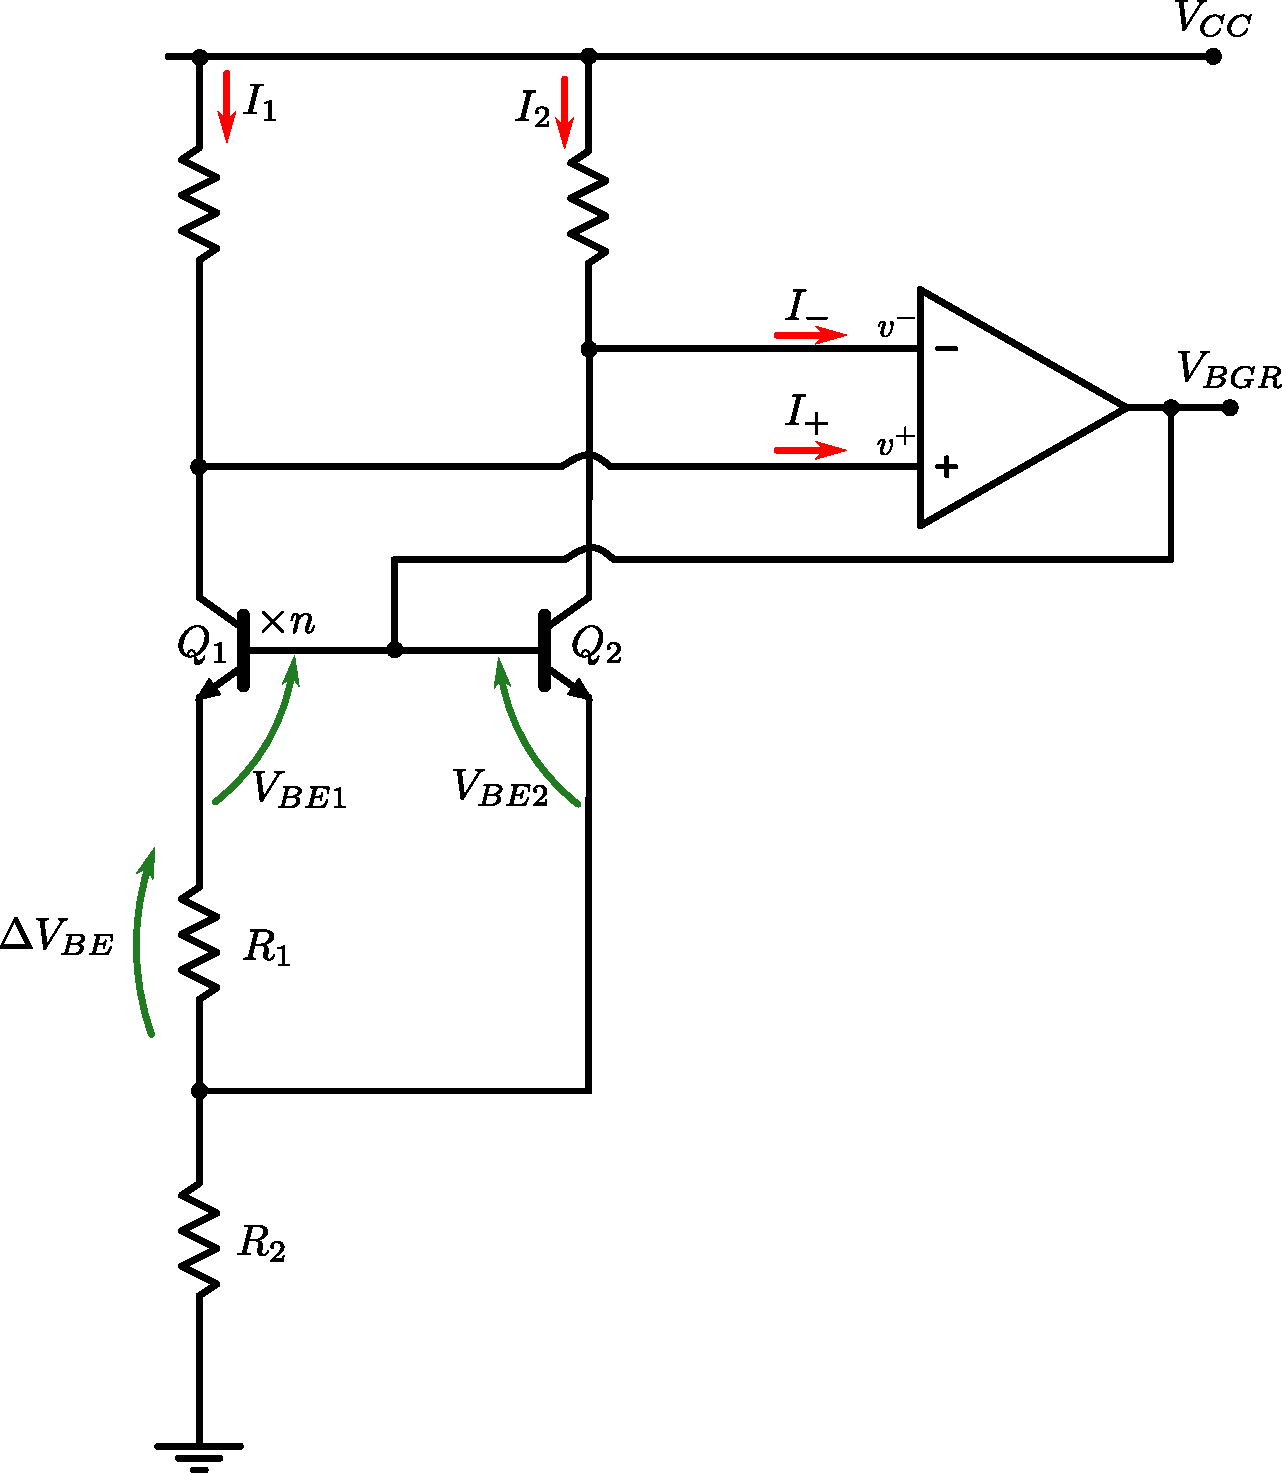
\includegraphics[width=0.5\linewidth]{Figures/BGRV-Brokaw.pdf}
	\caption{Brokow Bandgap Reference Voltage}
	\label{fig:brokaw} % !?
\end{figure}

Current inputs to OTA expected because of potential NPN $I_b$.

\subsection{Tsividis bandgap reference}

% Dependance on supply voltage?

\section{Errors PTAT or non-PTAT}
\begin{itemize}
    \item input DC opAmp offset, is very important paper used chopping to lower this dc offset.
    \item $V_{BE}$ diode connected
\end{itemize}

\newpage % Appendixlike

\section{PTAT Bias}

\begin{figure}[ht!]
	\centering
	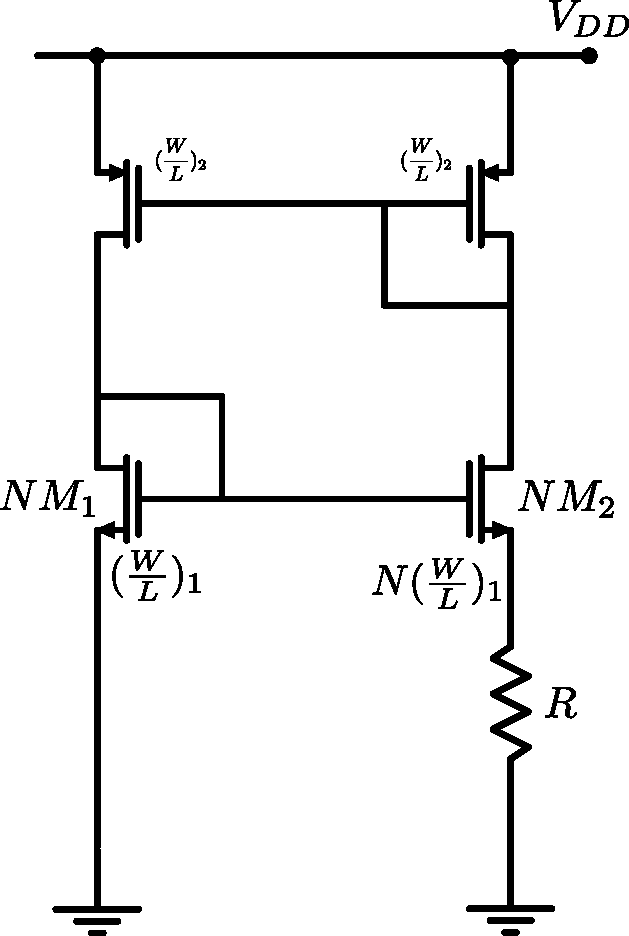
\includegraphics[width=0.35\linewidth]{Figures/PTAT-bias.pdf}
	\caption{PTAT Bias} % Proportional to absolute temperature Bias
	\label{fig:ptat-bias} 
\end{figure}

Only large signal analysis:

\begin{equation}
    V_{gs1} = V_{gs2} + R \, I_{D1}
\end{equation}

\begin{equation}
    I_{D1} = \mu_n C_{ox} \dfrac{W}{L}(V_{GS} - V_{th})^2
\end{equation}

Invert the function to $I_D = f(V_{GS})$:

\begin{equation}
    V_{GS}  = V_{th} + \sqrt{\dfrac{I_{D1}}{\mu_n C_{ox} \frac{W}{L}}}
\end{equation}

\textit{PMOS} mirror forces $I_{D1} = I_{D2}$:

\begin{align}
    V_{GS1}  = V_{th} + \sqrt{\dfrac{I_{D1}}{\mu_n C_{ox} \frac{W}{L}}},\\
    V_{GS2}  = V_{th} + \sqrt{\dfrac{I_{D2}}{\mu_n C_{ox} N \frac{W}{L}}}
\end{align}

Subtracting the 2 gate-source voltages: % Are threshold voltages the same?

\begin{equation}
    R \, I_{D1} = V_{GS1} - V_{GS2}  = (1 - \dfrac{1}{\sqrt{N}}) \sqrt{\dfrac{I_{D1}}{\mu_n C_{ox} \frac{W}{L}}}
\end{equation}

If we square both sides:

\begin{equation}
    I_{D1} = V_{GS1} - V_{GS2}  = (1 - \dfrac{1}{\sqrt{N}})^2 \dfrac{1}{R^2} \dfrac{1}{\mu_n C_{ox} \frac{W}{L}}
\end{equation}

\subsection{Start-up circuit}
\begin{figure}[ht!]
	\centering
	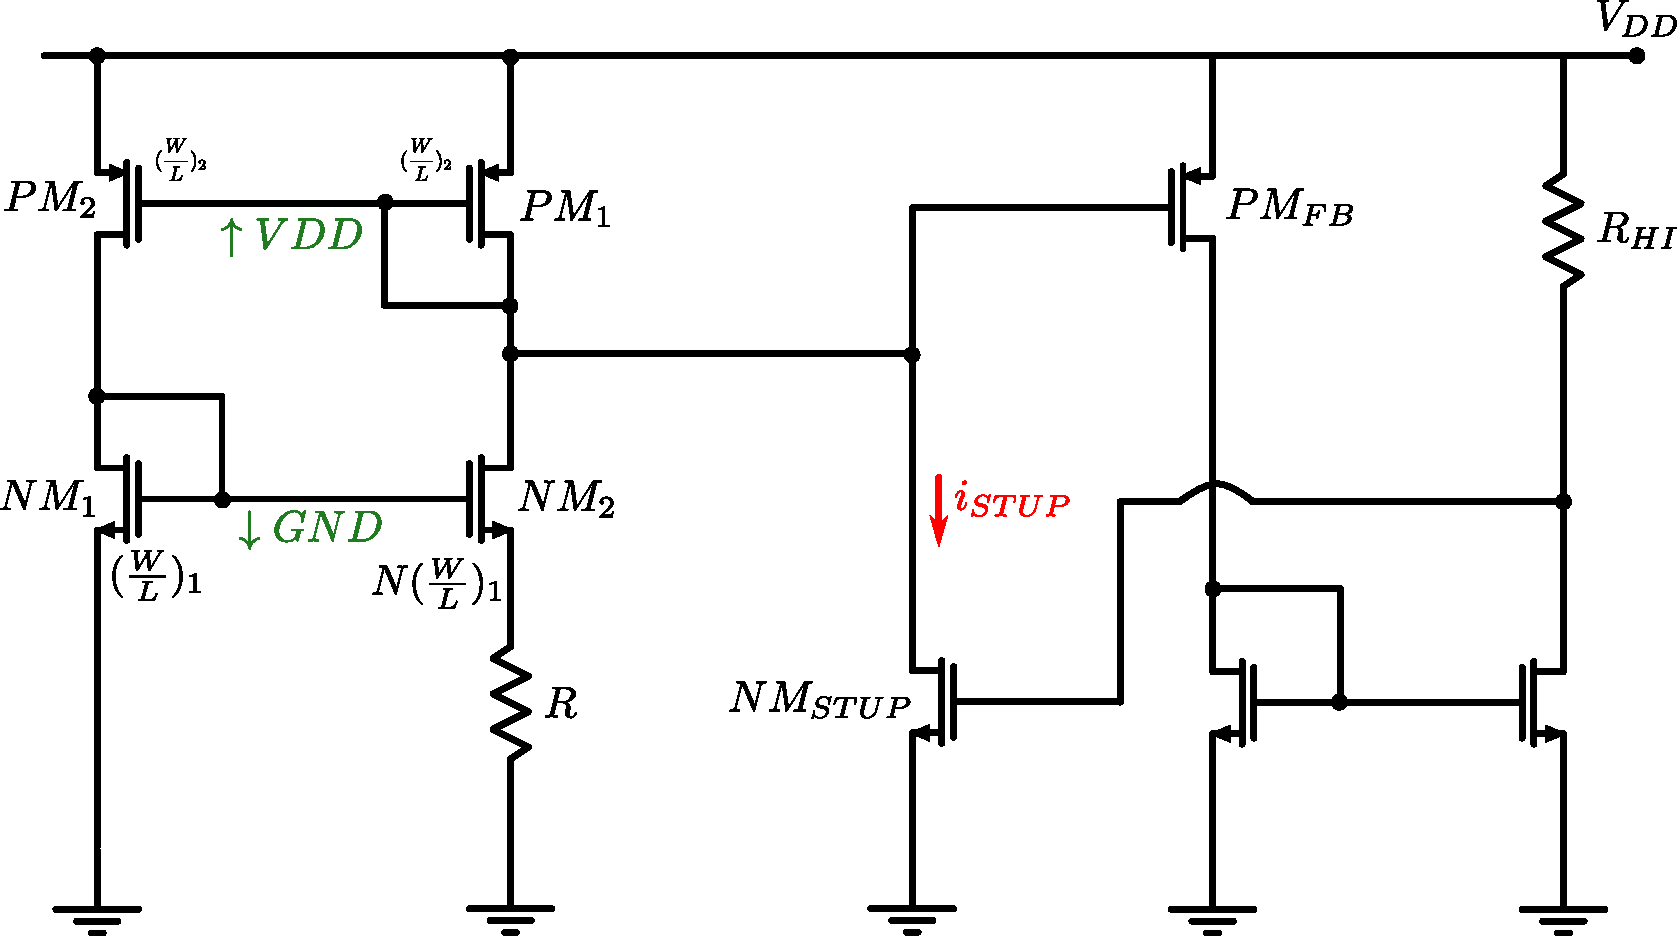
\includegraphics[width=0.7\linewidth]{Figures/PTAT-bias-startup.pdf}
	\caption{PTAT Bias Start-up Circuit TODO} % Proportional to absolute temperature Bias
	\label{fig:ptat-bias-startup} 
\end{figure}

% To check what it looks like?

\section{Bandgap Reference Design}

\begin{figure}[ht!]
	\centering
	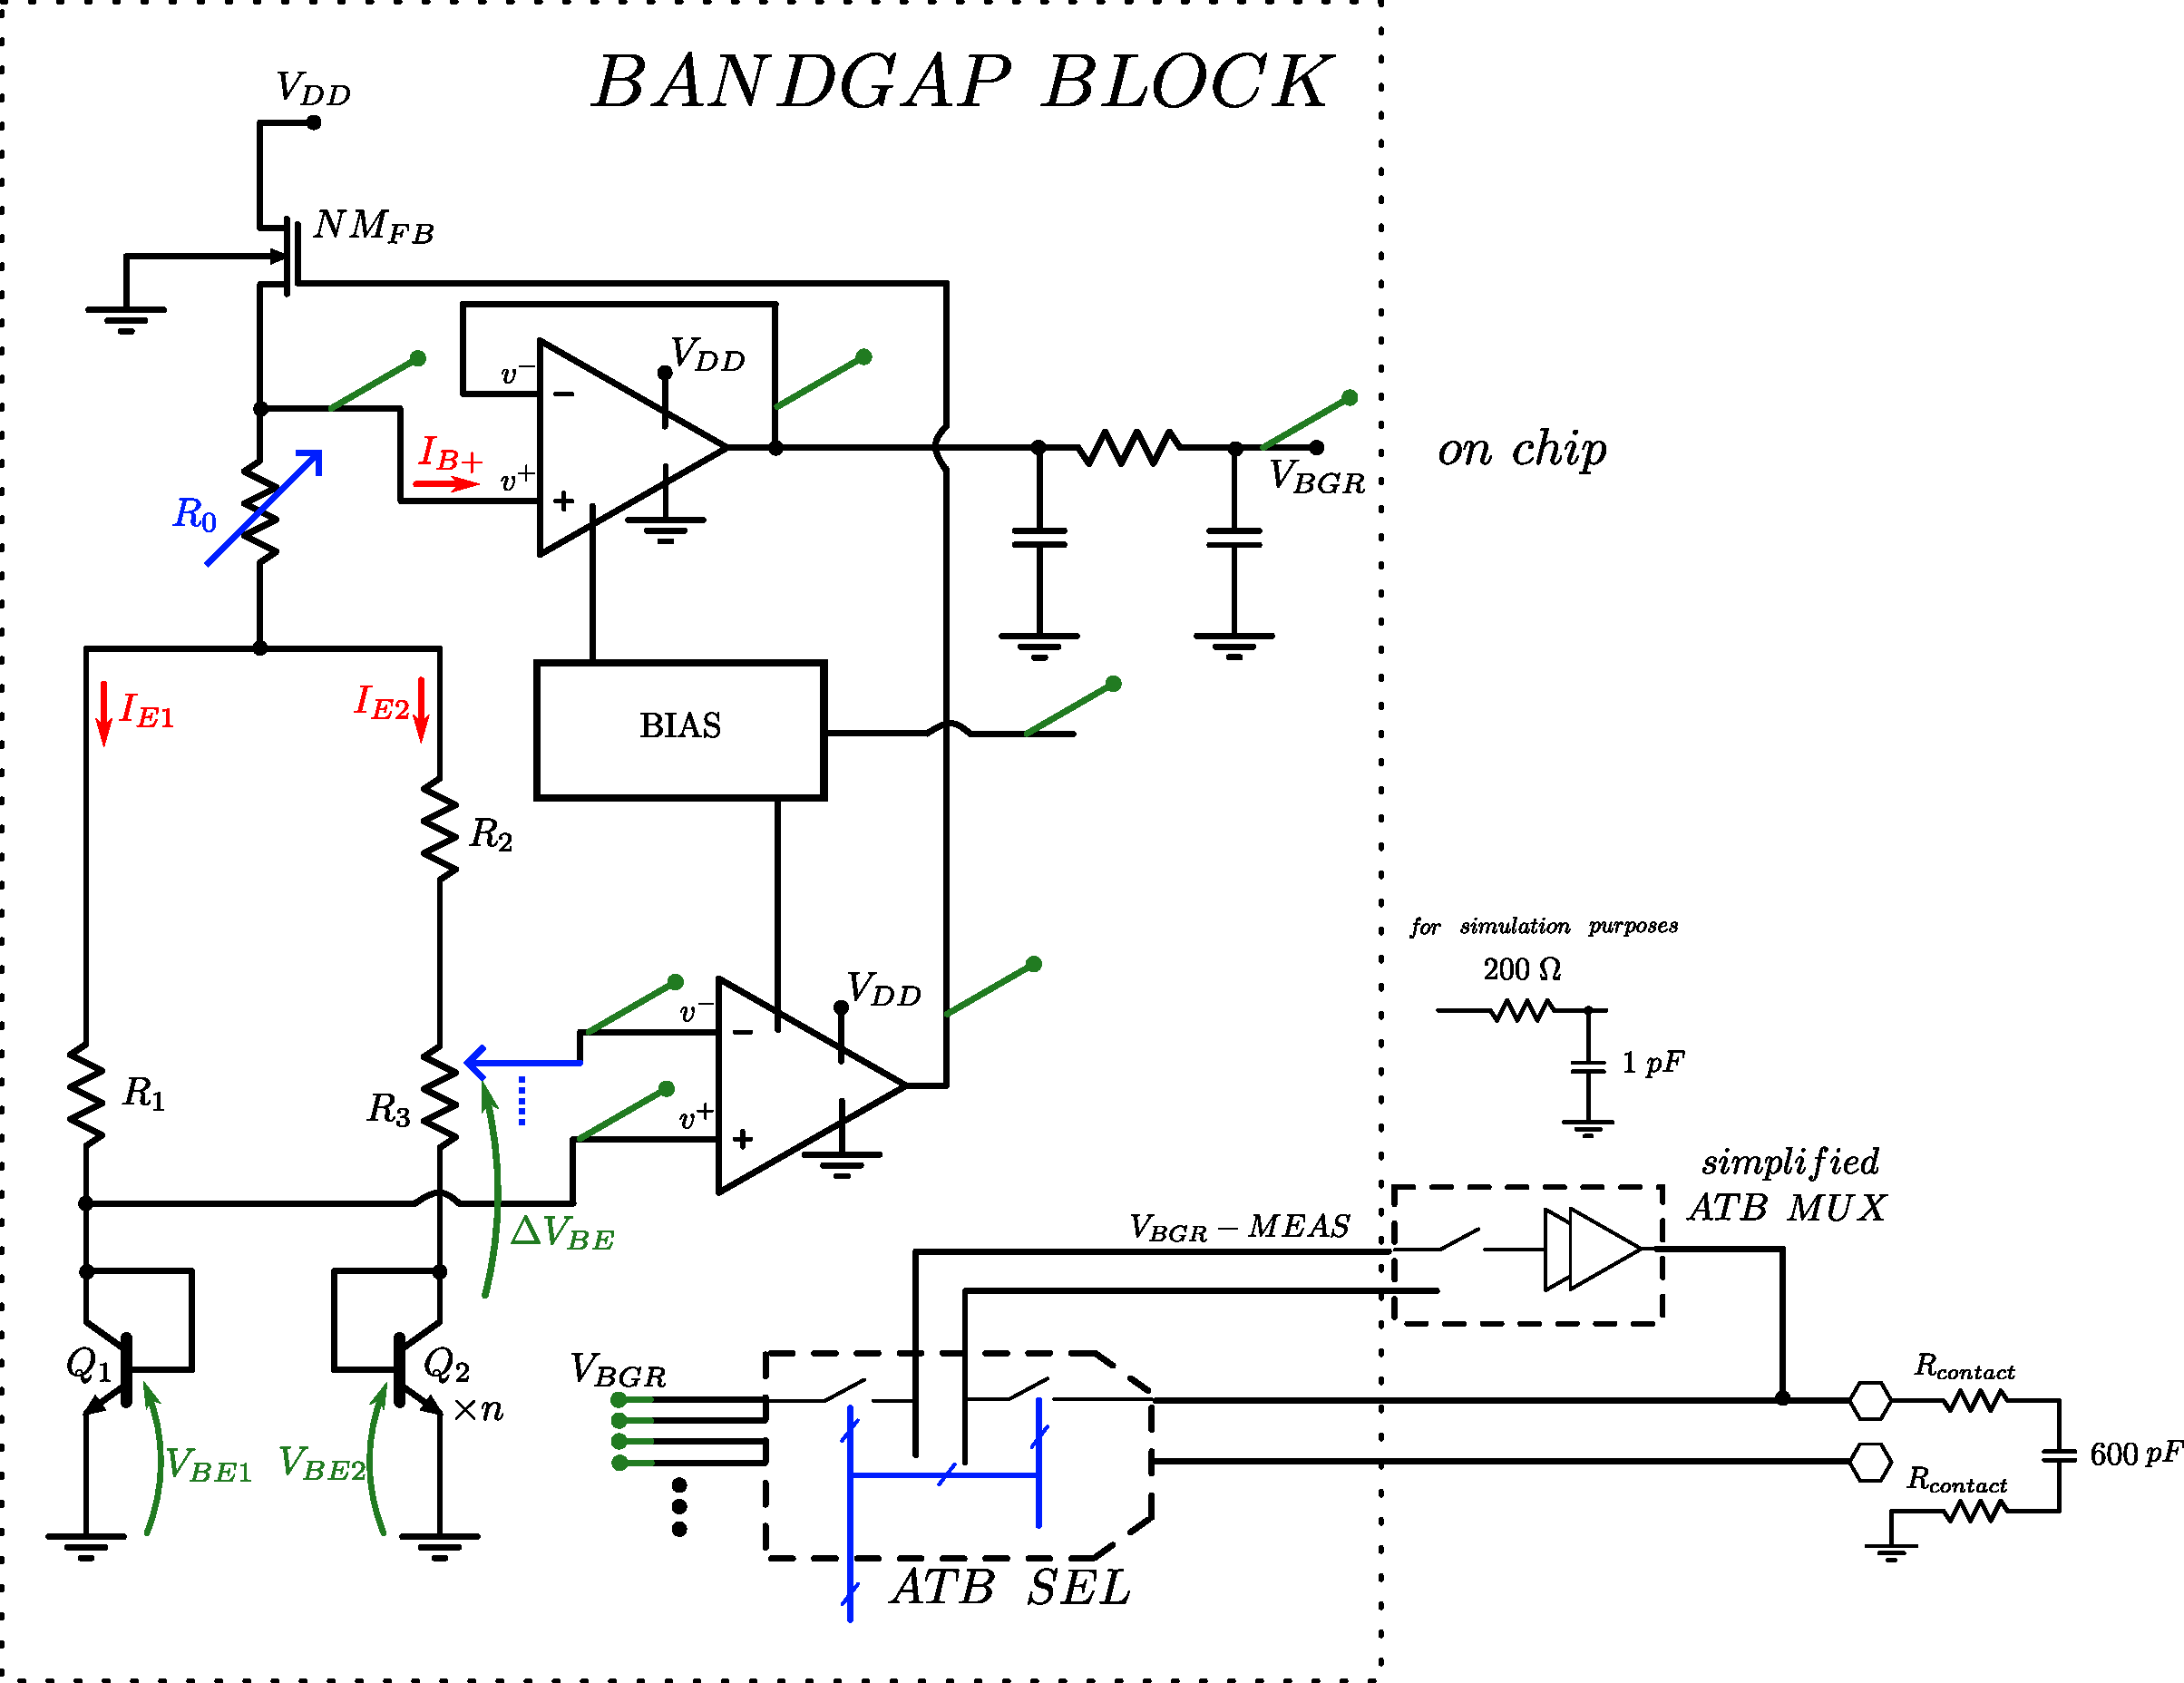
\includegraphics[width=0.5\linewidth]{Figures/BGRV-design.pdf}
	\caption{Bandgap Reference Voltage} % Proportional to absolute temperature Bias
	\label{fig:BGRV-design} 
\end{figure}


\section{Operational Transconductance Amplfiers Design}

Need to check saturation region, also subthreshold region or not.

\subsection{Comparator OTA}

Input differential pair is PMOS.

\subsection{Buffer OTA}
% Jedinični bafer
Expected input is around $1.3$ V. Transistor used for input differential pairs is npn BJT.


\subsection{Testing stability}

Identified three loops: feedback loop for comparator, buffer loop, and start-up circuit.




% \begin{itemize}[noitemsep]
% \item \uline{For Music:} The audio file for your submission in MP3 format.

% \end{itemize}

% \subsection{Illustrations and Media}

% For figures or illustrations, please upload them as PNG, JPEG, SVG, or TIFF files, and of a suitable standard to reproduce, at least 300 dpi. Full art preparation guidelines can be found \href{https://drive.google.com/file/d/1XBrYgYhOPmB3yAnfSL3PqGKXPNw0NAFE/view}{here}.

% If the images are not the work of the author, please begin acquiring images and clearing rights as soon as your article or review has been accepted. Permission instructions can be found \href{https://drive.google.com/file/d/1TJF59MuoX3erJv5WXY6jg1Uh0hZzYU6N/view}{here}; a template for requesting permissions is available \href{https://drive.google.com/file/d/1MJ9yFqoR7GNSpBaNPJLexXKvkF4yifzR/view}{here}.

% All images should be cleared for copyright purposes, and all costs and permissions to reproduce are the responsibility of the authors to provide correct credit lines for images and digital files. Online rights must be obtained from the rights-holder. openwork illustrates its digital publication in full color, although grayscale images may be accepted depending on the source material.

% The Journal encourages multimedia additions to its articles. Please submit a short comment to the editors describing any plans for incorporating media if not already clear from submitted materials.

% Copyright clearance and any associated costs for permissions for audio and video recordings, or other varieties of digital media, are the sole responsibility of the author.

% \section*{Article-Specific Preparation Guides}

% All texts should be original. Neither previously published work nor work under consideration for publication elsewhere will be accepted. Texts must be submitted in English.

% \subsection{Style}

% \subsubsection{House Style}
% Please adhere to the following house style preferences.
% \begin{itemize}[noitemsep]
%     \item All text should be single-spaced.
%     \item Paragraphs should be indicated by a line space, not indented or separated using paragraph spacing.
%     \item Boldface should not be used except for headings, and underlining should not be used.
%     \item In the main text, italicize titles of books and journals (please do not use underlining).
%     \item Put titles of articles, doctoral theses, and exhibitions in single inverted commas.
%     \item Figures and illustration references should be included in the text in parentheses (e.g., “(Fig. 2)”), and the captions should be numbered by order of appearance (not descriptively).
% 	\item Notes should be formatted as endnotes, with Arabic numerals.
%     \item spelling should conform to American English standards (e.g., color, center, recognize, etc.)
%     \item Quotations should be set within double inverted commas, and quotations within quotations in single inverted commas. Quotations more than six lines long should start on the next line and should be indented.
% \end{itemize}



% \subsection{Formatting}

% Please adhere to the following specifications for page layout and formatting by using the following template. Do not modify the template layout! Do not modify the line spacing!

% \subsubsection{Layout}
% \begin{itemize}[noitemsep]
%     \item Paper size must be standard US Letter.
%     \item Text must be written in one column. Multi-column layouts should not be used.
%     \item Margins should be 1 inch on all four sides.
%     \item Page headers must include a running head with the first author after the first page. 
%     \item Page footers must include the page number right-aligned on all pages. 
% \end{itemize}

% \subsubsection{Section headings}
% All headings must be left-aligned with boldface. Section headings should be 16 points and written in title case (i.e., every major word in the heading is capitalized). Sub-section headings should be 14 points and written in title case (i.e., every major word in the heading is capitalized). Sub-sub-section headings should be 12 points and written in sentence case (i.e., the first word is capitalized and the rest are in lowercase), with no extra line space separating the heading from the first paragraph. No more than three levels of headings should be used.

% \subsubsection{Fonts}
% The main text must be written using Times New Roman font. Standard body text should be 12 points, while the title should be 18 points. Other font types may be used if needed for special notations or equations.

% \subsection{Figures}

% Figures must be centered on the page. Figures that span the width of the page must be included on the top or bottom of the page. A minimum font size of 8 points is recommended for all text within figures. Please do not use stipple fill patterns as they do not render correctly in Adobe PDF.

% \subsection{Tables}

% Tables must be centered on the page. A minimum font size of 8 points is recommended for all text within tables. An example of a table is shown below.
% \begin{table*}[hbt!]
%     \centering
%     \begin{tblr}{c|c}
%         \toprule
%         \textbf{Note Name} & \textbf{Frequency (Hz)} \\
%         \midrule
%         F4 & 349.23 \\
%         \midrule
%         G4 & 392 \\
%         \midrule
%         A4 & 440 \\
%         \midrule
%         B4 & 493.88 \\
%         \midrule
%         C5 & 523.25 \\
%         \bottomrule
%     \end{tblr}
%     \caption{Note names and their corresponding frequencies.}
% \end{table*}

% \subsection{Captions}

% Captions should follow each figure or table and conform to the guidelines below:

% \begin{itemize}[noitemsep]
%     \item Please number figures and tables in order and make sure that image files can be clearly identified from their filenames.
%     \item Images not created by the author must have a catalogue-style caption supplied as a separate list. Captions should include:
%     \begin{itemize}[noitemsep]
%         \item [$\circ$] Maker
%         \item [$\circ$] Title (in italics)
%         \item [$\circ$] Date
%         \item [$\circ$] Medium
%         \item [$\circ$] Measurements
%         \item [$\circ$] Location (Institution, Geographic Location)
%         \item [$\circ$] Copyright statement
%         \item [$\circ$] Courtesy line and/or photo credit
%     \end{itemize}
% \end{itemize}

% An example of a caption is shown below: 

% \textbf{Fig 1.} Yinka Shonibare, The Swing (after Fragonard), 2001, mannequin, cotton costume, 2 slippers, swing seat, 2 ropes, oak twig and artificial foliage, 3.3 x 3.5 x 2.2 m (Tate, London) © Yinka Shonibare; image courtesy Stephen Friedman Gallery, London.

% \subsection{Equations}

% Equations should be placed on separate lines and numbered. An example is shown below.

% \begin{equation}
% f(x) = a_0 + \sum_{n=1}^{\infty} \left( a_n \cos\frac{n\pi x}{L} + b_n \sin\frac{n\pi x}{L} \right)
% \end{equation}

% \section{Submission Checklist}

% Prior to submitting your proposal to openwork, please verify that you have completed all of the items in the checklist below.

% \begin{itemize}[noitemsep]
%     \item The submission adheres to the Submission Guidelines and Article-Specific Preparation Guidelines (if applicable) outlined in the sections above.
%     \item All identifying information (name, affiliation, etc.) is removed from texts, metadata, and associated media.
%     \item Where available, URLs for the references have been provided.
%     \item The author accepts responsibility for obtaining permission to publish any media submitted per the Submission Guidelines.
%     \item The submission has not been previously published, nor has it been before another journal for consideration.
%     \item The author grants the Journal the authority to publish the article as an Open Access article distributed under the terms of \href{https://creativecommons.org/licenses/by-nc-nd/4.0/}{Creative Commons Attribution, NonCommercial, NoDerivatives license (CC BY-NC-ND).} 
% \end{itemize}

% \bibliography{references}

% \printbibliography

\end{document}